\documentclass[12pt,letter]{article} 

%%%%%%%%%%%%%%%%%%%%%%%%%%%%%%%%%%%%%%%%%%%%%%%%%%
%%%%%%%%%%%%%%%%%%%% PREAMBLE %%%%%%%%%%%%%%%%%%%%
%%%%%%%%%%%%%%%%%%%%%%%%%%%%%%%%%%%%%%%%%%%%%%%%%%


% -------------------- defaults -------------------- %
% load lots o' packages

% layout control
\usepackage[paper=a4paper,left=25mm,right=25mm,top=20mm,bottom=25mm]{geometry}
\usepackage[onehalfspacing]{setspace}
\setlength{\parskip}{.5em}
\usepackage{rotating}
\usepackage{setspace}
\usepackage{fancyhdr}	
\usepackage{parallel}
\usepackage{parcolumns}

% math typesetting
\usepackage{array}
\usepackage{amsmath}
\usepackage{amssymb}
\usepackage{amsfonts}
\usepackage{relsize}

\usepackage{verbatim}

% restricts float objects to be inserted before end of section
% creates float barriers
\usepackage[section]{placeins}

% tables
\usepackage{tabularx}
\usepackage{booktabs}
\usepackage{multicol}
\usepackage{multirow}
\usepackage{longtable}

\usepackage[%
decimalsymbol=.,
digitsep=fullstop
]{siunitx}

% to adapt caption style
\usepackage[font={small},labelfont=bf]{caption}

% references
\usepackage[longnamesfirst]{natbib}
\bibpunct{(}{)}{;}{a}{}{,}

% footnotes at bottom
\usepackage[bottom]{footmisc}

% to change enumeration symbols begin{enumerate}[(a)]
\usepackage{enumerate}

% to make enumerations and itemizations within paragraphs or
% lines. f.i. begin{inparaenum} for (a) is (b) and (c)
\usepackage{paralist}

% to colorize links in document. See color specification below
\usepackage[pdftex,hyperref,x11names]{xcolor}

% for multiple references and insertion of the word "figure" or "table"
% \usepackage{cleveref}

% load the hyper-references package and set document info
\usepackage[pdftex]{hyperref}

% graphics stuff
\usepackage{subfig}
\usepackage{graphicx}
\usepackage[space]{grffile} % allows us to specify directories that have spaces
\usepackage{placeins} % prevents floats from moving past a \FloatBarrier
%\usepackage{tikz}
% \usepackage{pgfplots}

% define clickable links and their colors
\hypersetup{%
unicode=false,          % non-Latin characters in Acrobat's bookmarks
pdftoolbar=true,        % show Acrobat's toolbar?
pdfmenubar=true,        % show Acrobat's menu?
pdffitwindow=false,     % window fit to page when opened
pdfstartview={FitH},    % fits the width of the page to the window
pdfnewwindow=true,%
pagebackref=false,%
pdfauthor={Shahryar Minhas},%
pdftitle={Title},%
colorlinks,%
citecolor=black,%
filecolor=black,%
linkcolor=black,%
urlcolor=RoyalBlue4}

% Including External Code
\usepackage{verbatim}
\usepackage{listings}
\lstset{
	language=R,
	basicstyle=\scriptsize\ttfamily,
	commentstyle=\ttfamily\color{gray},
	numbers=left,
	numberstyle=\ttfamily\color{gray}\footnotesize,
	stepnumber=1,
	numbersep=5pt,
	backgroundcolor=\color{white},
	showspaces=false,
	showstringspaces=false,
	showtabs=false,
	frame=single,
	tabsize=2,
	captionpos=b,
	breaklines=true,
	breakatwhitespace=false,
	title=\lstname,
	escapeinside={},
	keywordstyle={},
	morekeywords={}
	}

% -------------------------------------------------- %


% -------------------- title -------------------- %

\title{Title}
\vspace{\baselineskip}
\author{Shahryar Minhas}
\date{\today}

\setlength{\headheight}{15pt}
\setlength{\headsep}{20pt}
\pagestyle{fancyplain}
 
\fancyhf{}
 
\lhead{\fancyplain{}{Shahryar Minhas}}
\chead{\fancyplain{}{Header Title}}
\rhead{\fancyplain{}{\today}}
\rfoot{\fancyplain{}{\thepage}}

% ----------------------------------------------- %


% -------------------- customizations -------------------- %

% define the includegraphics search path
\graphicspath{{Graphics/}}

% easy commands for number propers
\newcommand{\first}{$1^{\text{st}}$}
\newcommand{\second}{$2^{\text{nd}}$}
\newcommand{\third}{$3^{\text{rd}}$}
\newcommand{\nth}[1]{${#1}^{\text{th}}$}

% easy command for boldface math symbols
\newcommand{\mbs}[1]{\boldsymbol{#1}}

% define bibliography style
\bibliographystyle{/Users/janus829/Documents/APSR}

% -------------------------------------------------------- %


%%%%%%%%%%%%%%%%%%%%%%%%%%%%%%%%%%%%%%%%%%%%%%%%%%
%%%%%%%%%%%%%%%%%%%% DOCUMENT %%%%%%%%%%%%%%%%%%%%
%%%%%%%%%%%%%%%%%%%%%%%%%%%%%%%%%%%%%%%%%%%%%%%%%%

% \doublespacing 

\begin{document}

% \maketitle

popularity of network approaches in recent years isq special issue...

notable work by cranmer on ergms re lsm

set of important challenges for lsm

relation to actual literature on lsm

we show...

\section{Replication Results}

% latex table generated in R 3.3.1 by xtable 1.8-2 package
% Sun Aug 21 03:32:43 2016
\begin{table}[ht]
\centering
\begingroup\normalsize
\begin{tabular}{lccccc}
   & Logit & MRQAP & LSM & ERGM & AME \\ 
  \hline
\hline
Intercept/Edges & -4.44$^{\ast}$ & -4.24$^{\ast}$ & 0.94$^{\ast}$ & -12.17$^{\ast}$ & -3.39$^{\ast}$ \\ 
   & (0.34) &  & [0.09; 1.82] & (1.40) & [-4.38; -2.50] \\ 
  \textbf{Conflicting policy preferences} &  &  &  &  &  \\ 
  $\;\;\;\;$ Business vs. NGO & -0.86 & -0.87$^{\ast}$ & -1.37$^{\ast}$ & -1.11$^{\ast}$ & -1.37$^{\ast}$ \\ 
   & (0.46) &  & [-2.42; -0.41] & (0.51) & [-2.44; -0.47] \\ 
  $\;\;\;\;$ Opposition/alliance & 1.21$^{\ast}$ & 1.14$^{\ast}$ & 0.00 & 1.22$^{\ast}$ & 1.08$^{\ast}$ \\ 
   & (0.20) &  & [-0.40; 0.39] & (0.20) & [0.72; 1.47] \\ 
  $\;\;\;\;$ Preference dissimilarity & -0.07 & -0.60 & -1.76$^{\ast}$ & -0.44 & -0.79$^{\ast}$ \\ 
   & (0.37) &  & [-2.62; -0.90] & (0.39) & [-1.55; -0.08] \\ 
  \textbf{Transaction costs} &  &  &  &  &  \\ 
  $\;\;\;\;$ Joint forum participation & 0.88$^{\ast}$ & 0.75$^{\ast}$ & 1.51$^{\ast}$ & 0.90$^{\ast}$ & 0.92$^{\ast}$ \\ 
   & (0.27) &  & [0.86; 2.17] & (0.28) & [0.40; 1.47] \\ 
  \textbf{Influence} &  &  &  &  &  \\ 
  $\;\;\;\;$ Influence attribution & 1.20$^{\ast}$ & 1.29$^{\ast}$ & 0.08 & 1.00$^{\ast}$ & 1.09$^{\ast}$ \\ 
   & (0.22) &  & [-0.40; 0.55] & (0.21) & [0.69; 1.53] \\ 
  $\;\;\;\;$ Alter's influence indegree & 0.10$^{\ast}$ & 0.11$^{\ast}$ & 0.01 & 0.21$^{\ast}$ & 0.11$^{\ast}$ \\ 
   & (0.02) &  & [-0.03; 0.04] & (0.04) & [0.07; 0.15] \\ 
  $\;\;\;\;$ Influence absolute diff. & -0.03$^{\ast}$ & -0.06$^{\ast}$ & 0.04 & -0.05$^{\ast}$ & -0.07$^{\ast}$ \\ 
   & (0.02) &  & [-0.01; 0.09] & (0.01) & [-0.11; -0.03] \\ 
  $\;\;\;\;$ Alter = Government actor & 0.63$^{\ast}$ & 0.68 & -0.46 & 1.04$^{\ast}$ & 0.55 \\ 
   & (0.25) &  & [-1.08; 0.14] & (0.34) & [-0.07; 1.15] \\ 
  \textbf{Functional requirements} &  &  &  &  &  \\ 
  $\;\;\;\;$ Ego = Environmental NGO & 0.88$^{\ast}$ & 0.99 & -0.60 & 0.79$^{\ast}$ & 0.67 \\ 
   & (0.26) &  & [-1.32; 0.09] & (0.17) & [-0.38; 1.71] \\ 
  $\;\;\;\;$ Same actor type & 0.74$^{\ast}$ & 1.12$^{\ast}$ & 1.17$^{\ast}$ & 0.99$^{\ast}$ & 1.04$^{\ast}$ \\ 
   & (0.22) &  & [0.63; 1.71] & (0.23) & [0.63; 1.50] \\ 
  \textbf{Endogenous dependencies} &  &  &  &  &  \\ 
  $\;\;\;\;$ Mutuality & 1.22$^{\ast}$ & 1.00$^{\ast}$ &  & 0.81$^{\ast}$ & 0.39 \\ 
   & (0.21) &  &  & (0.25) & [-0.12; 0.96] \\ 
  $\;\;\;\;$ Outdegree popularity &  &  &  & 0.95$^{\ast}$ &  \\ 
   &  &  &  & (0.09) &  \\ 
  $\;\;\;\;$ Twopaths &  &  &  & -0.04$^{\ast}$ &  \\ 
   &  &  &  & (0.02) &  \\ 
  $\;\;\;\;$ GWIdegree (2.0) &  &  &  & 3.42$^{\ast}$ &  \\ 
   &  &  &  & (1.47) &  \\ 
  $\;\;\;\;$ GWESP (1.0) &  &  &  & 0.58$^{\ast}$ &  \\ 
   &  &  &  & (0.16) &  \\ 
  $\;\;\;\;$ GWOdegree (0.5) &  &  &  & 8.42$^{\ast}$ &  \\ 
   &  &  &  & (2.11) &  \\ 
   \hline
\hline
\end{tabular}
\endgroup
\caption{* p $<$ 0.05. Logistic regression and ERGM results are shown with standard errors in parentheses. MRQAP provides no standard errors. LSM and AME are shown with 95\% posterior credible intervals provided in brackets.} 
\label{tab:regTable}
\end{table}


\section{Capturing Network Stuff}

\begin{figure}[ht]
	\centering
	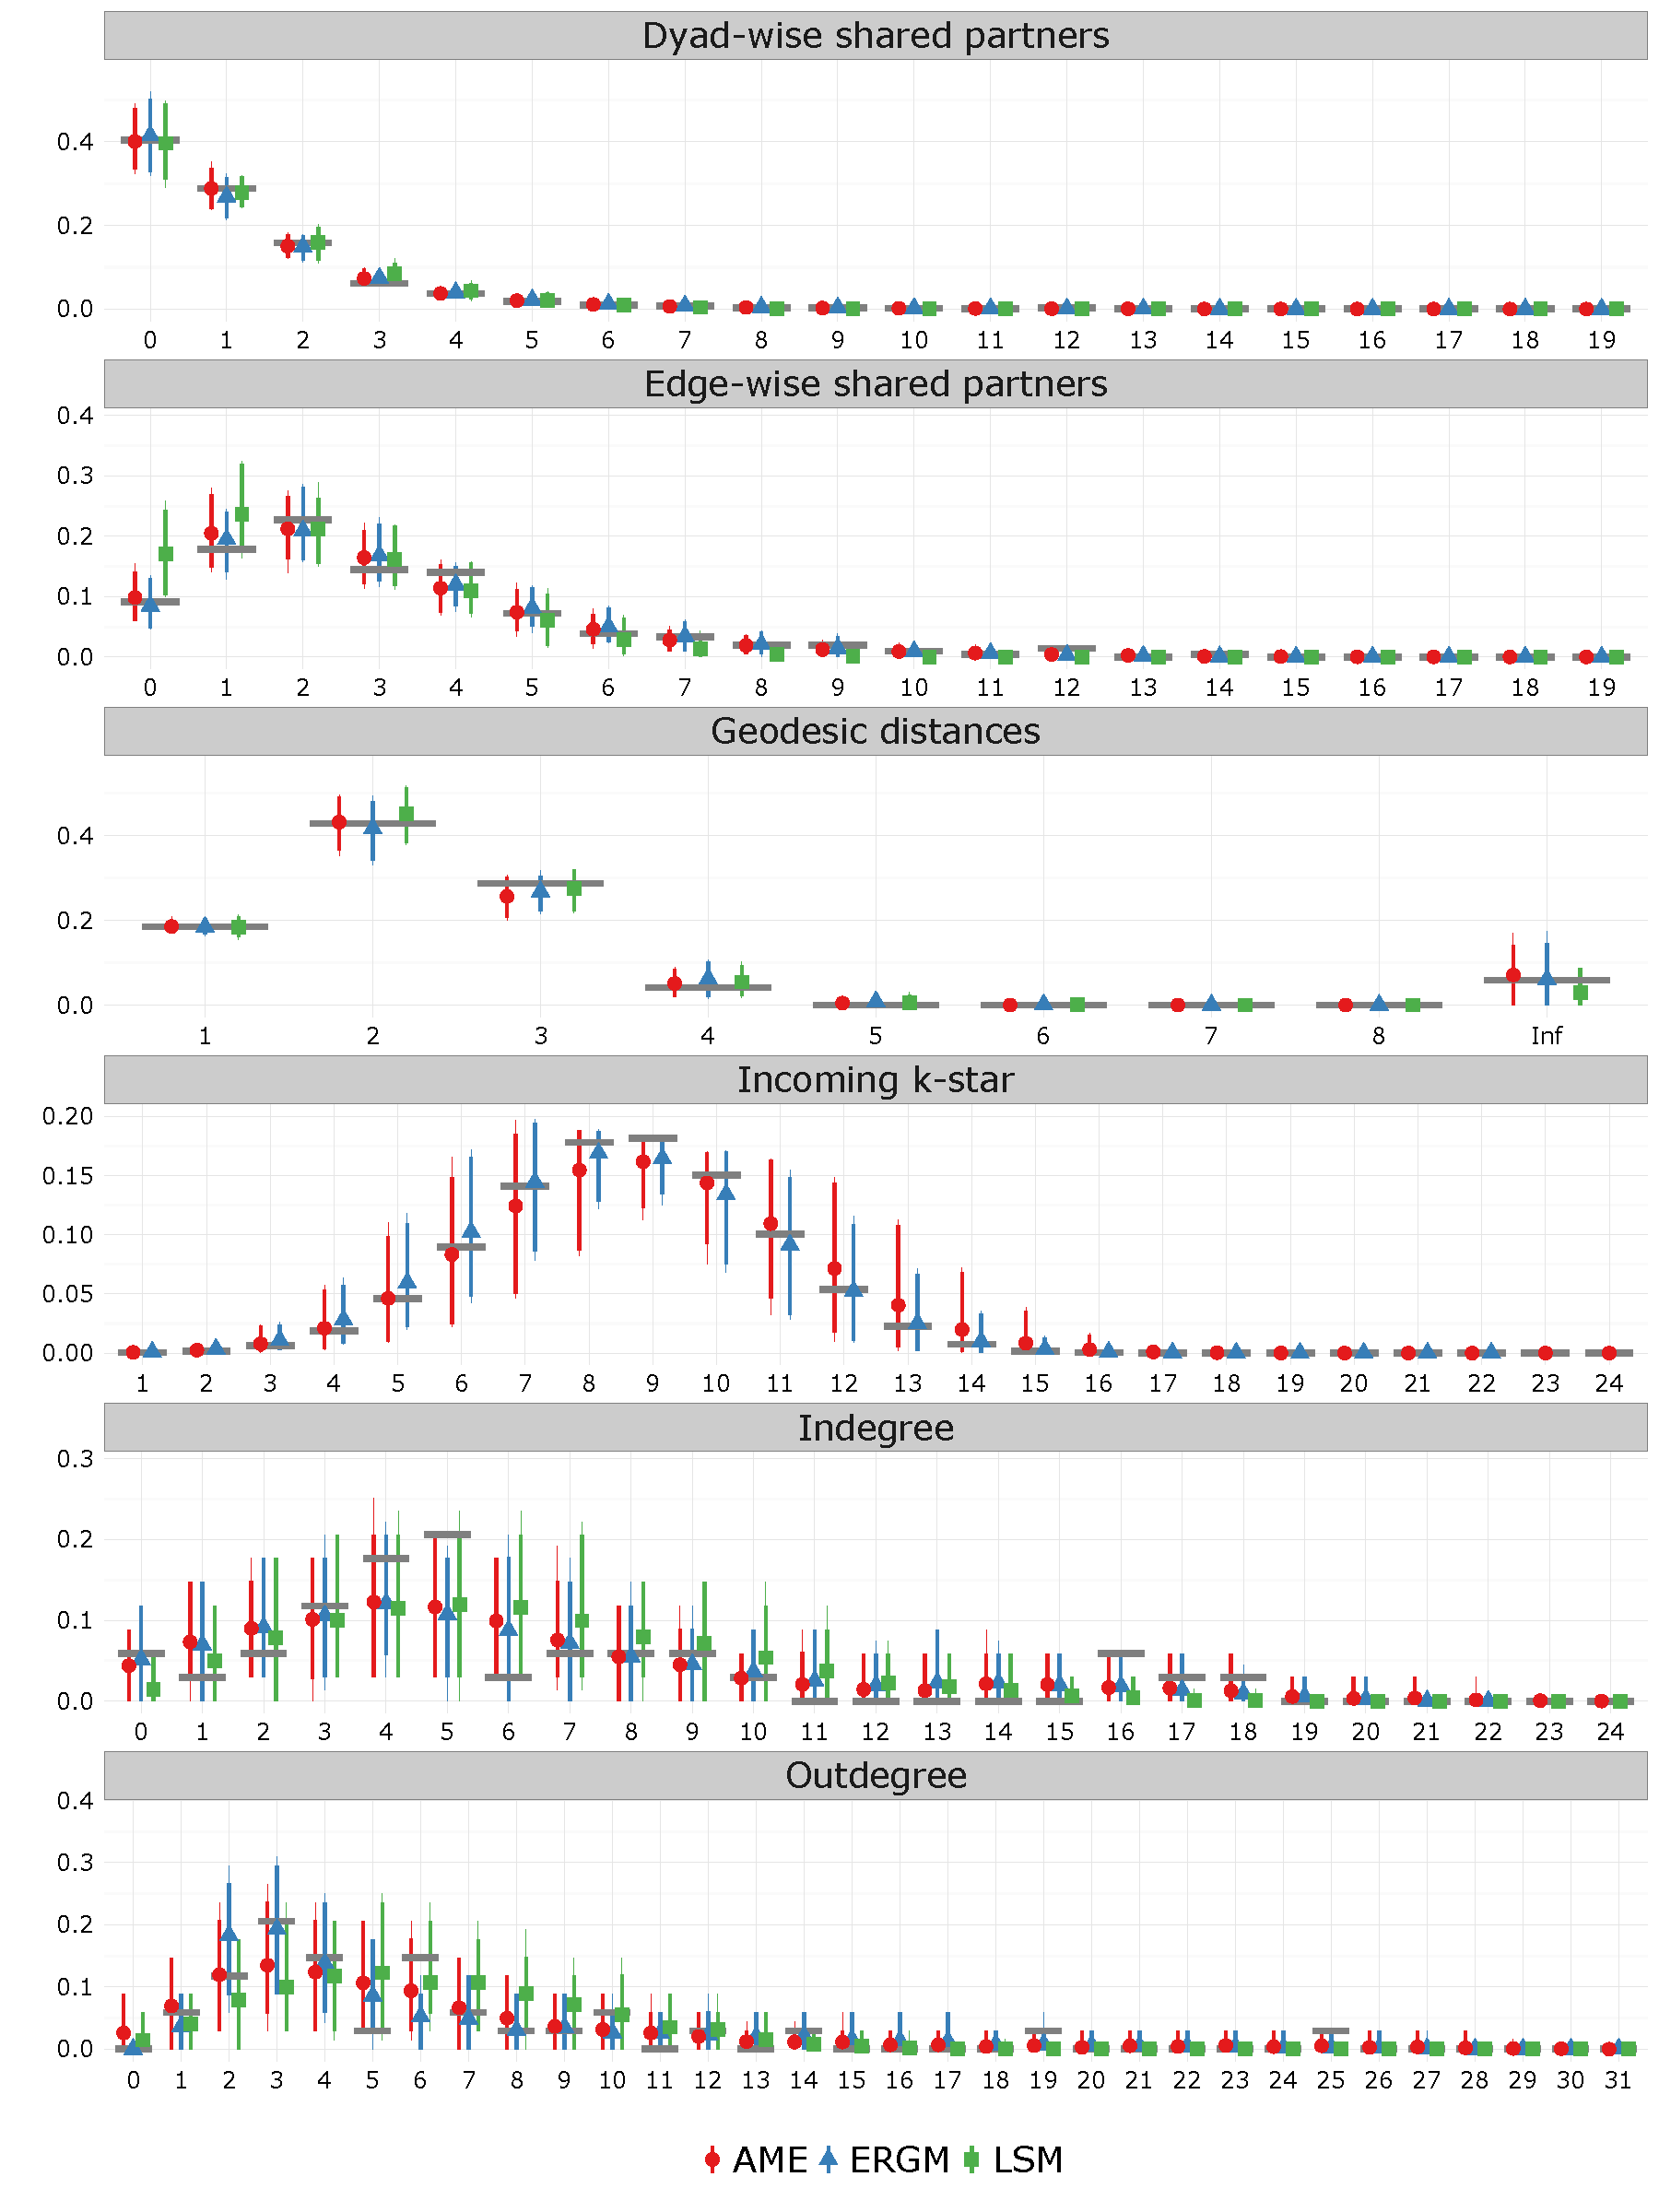
\includegraphics[width=1\textwidth]{ggGofAll}
	\caption{network stats }
	\label{fig:gofAll}
\end{figure}

Figure~\ref{fig:ergmAmePerf} give posterior predictive goodness of fit summaries for four network statistics: (1) the empirical standard deviation of the row means; (2) the empirical stan- dard deviation of the column means; (3) the empirical within-dyad correlation; (4) a normalized measure of triadic dependence

\begin{figure}[ht]
	\centering
	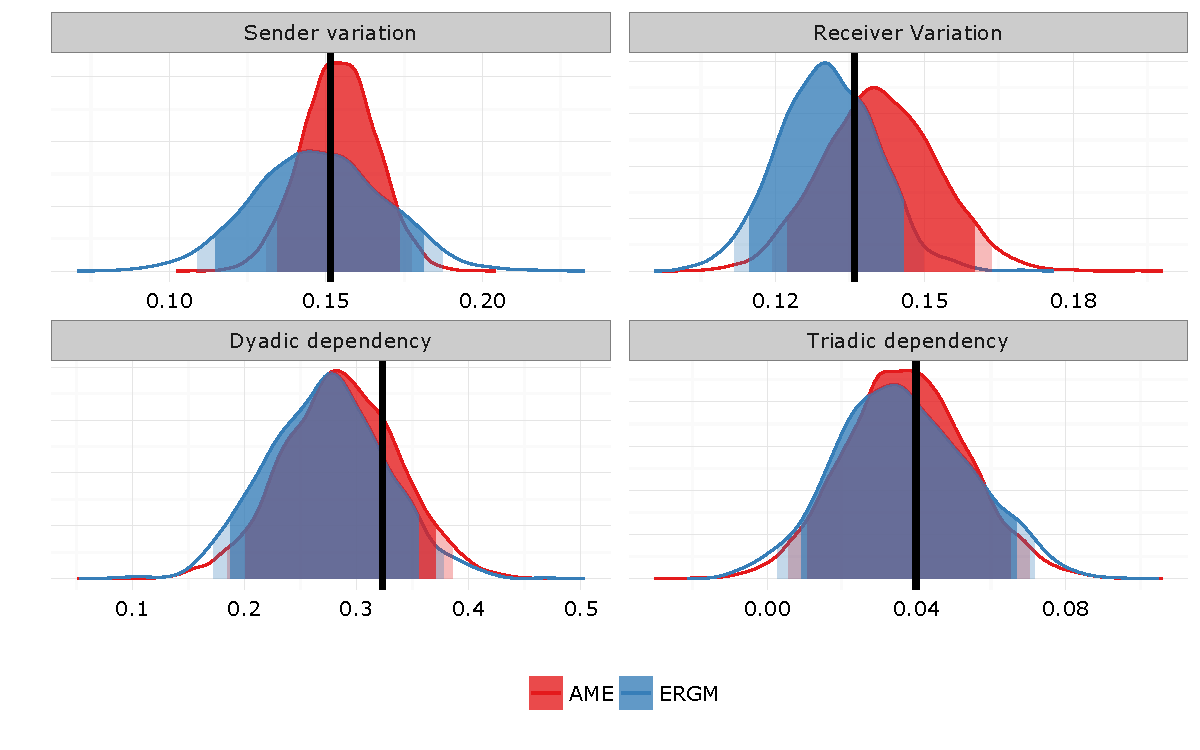
\includegraphics[width=1\textwidth]{ergmAmePerf}
	\caption{Posterior predictive goodness of fit summary}
	\label{fig:ergmAmePerf}
\end{figure}

\section{Tie Formation Prediction}

% latex table generated in R 3.3.1 by xtable 1.8-2 package
% Tue Oct 18 00:16:48 2016
\begin{table}[ht]
\centering
\begingroup\normalsize
\begin{tabular}{lcc}
  & AUC & AUC (PR) \\ 
  \hline
\hline
AME & 0.99 & 0.94 \\ 
  LSM & 0.92 & 0.68 \\ 
  ERGM & 0.91 & 0.70 \\ 
  MRQAP & 0.88 & 0.67 \\ 
  Logit & 0.88 & 0.67 \\ 
  \end{tabular}
\endgroup
\caption{Area under the curve (AUC) comparison.} 
\label{tab:aucTable}
\end{table}


\begin{figure}[ht]
	\centering
	\begin{tabular}{cc}
	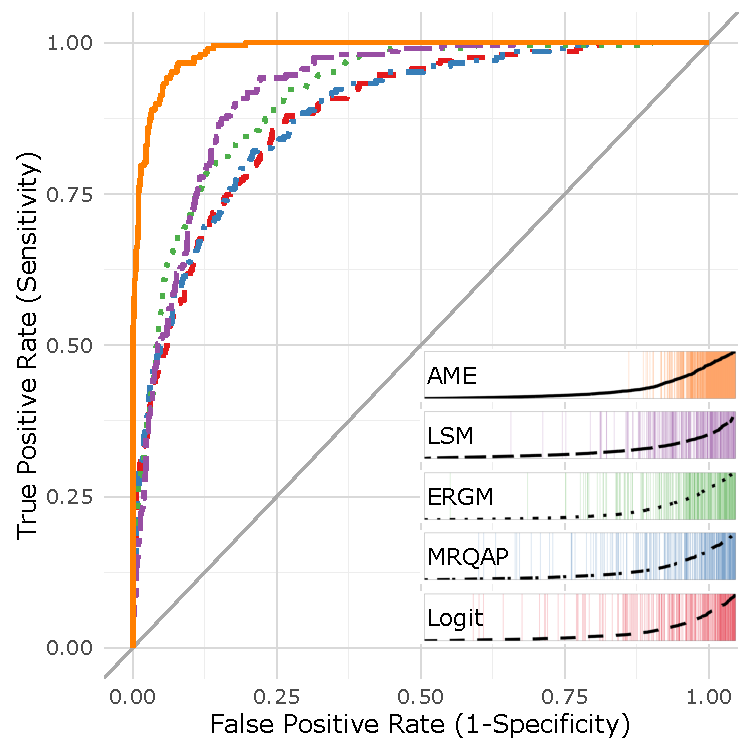
\includegraphics[width=.5\textwidth]{roc} & 
	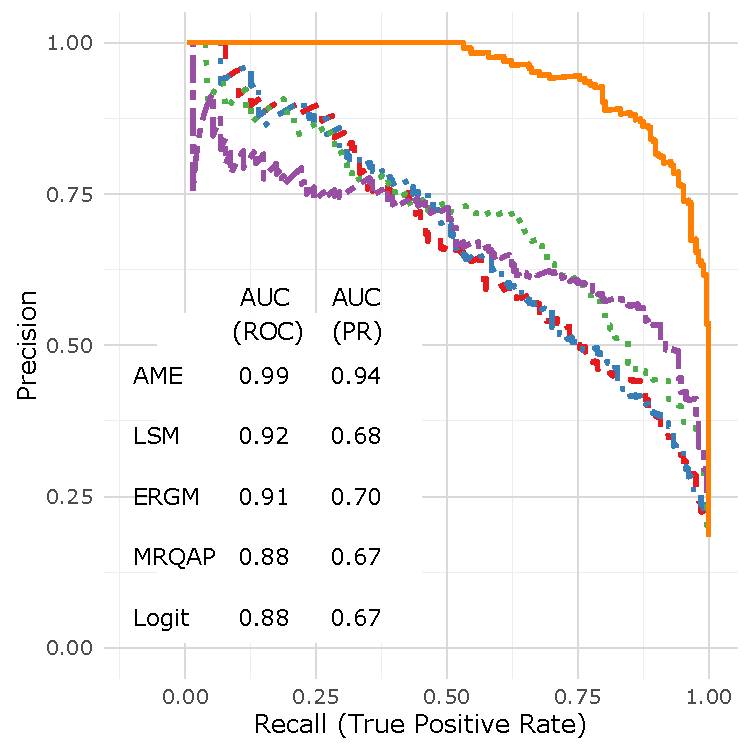
\includegraphics[width=.5\textwidth]{rocPr}	
	\end{tabular}
	\caption{ROC and separation plots}
	\label{fig:roc}
\end{figure}

\section{Conclusion}


\newpage
\section{Appendix}

\section{AMEN Model Convergence}

\begin{figure}[ht]
	\centering
	\begin{tabular}{cc}
	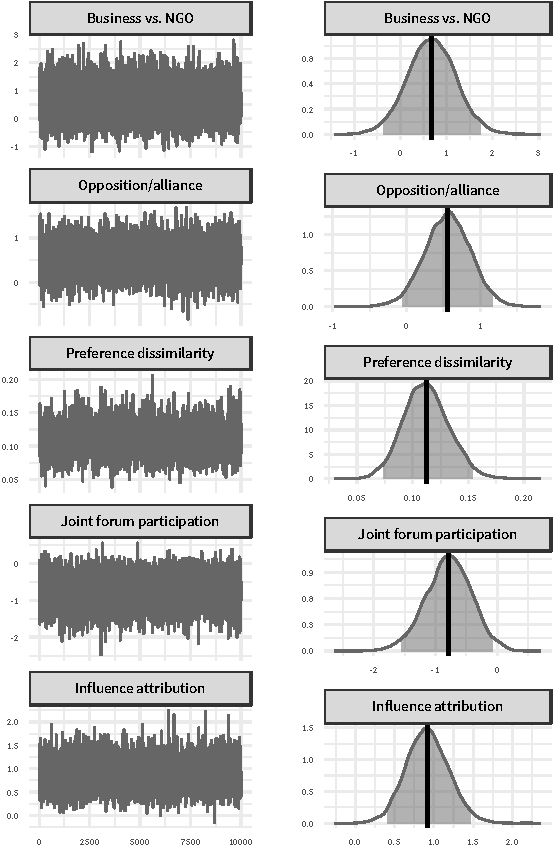
\includegraphics[width=.45\textwidth]{ameConv1_SR2} &
	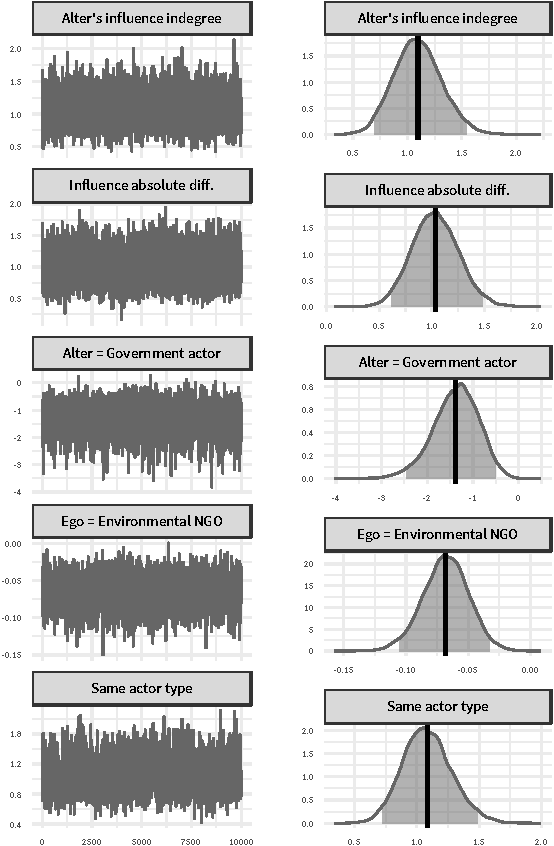
\includegraphics[width=.45\textwidth]{ameConv2_SR2}
	\end{tabular}
	\caption{ame convergence}
	\label{fig:ameConv}
\end{figure}


\section{Comparison with other AME Parameterizations}

% latex table generated in R 3.3.1 by xtable 1.8-2 package
% Sun Aug 21 03:38:29 2016
\begin{table}[ht]
\centering
\begingroup\tiny
\begin{tabular}{lccccc}
   & AME (k=0) & AME (k=1) & AME (k=2) & AME (k=3) & AME (k=4) \\ 
  \hline
\hline
Intercept/Edges & -2.19$^{\ast}$ & -2.72$^{\ast}$ & -2.75$^{\ast}$ & -2.92$^{\ast}$ & -3.03$^{\ast}$ \\ 
   & [-2.55; -1.85] & [-3.41; -1.82] & [-3.59; -1.88] & [-3.81; -2.04] & [-4.03; -1.99] \\ 
  \textbf{Conflicting policy preferences} &  &  &  &  &  \\ 
  $\;\;\;\;$ Business vs. NGO & -0.46 & -0.88$^{\ast}$ & -0.96$^{\ast}$ & -1.03$^{\ast}$ & -1.12$^{\ast}$ \\ 
   & [-0.95; -0.01] & [-1.64; -0.22] & [-1.86; -0.22] & [-1.96; -0.24] & [-2.15; -0.25] \\ 
  $\;\;\;\;$ Opposition/alliance & 0.65$^{\ast}$ & 0.79$^{\ast}$ & 0.86$^{\ast}$ & 0.95$^{\ast}$ & 1.03$^{\ast}$ \\ 
   & [0.44; 0.86] & [0.53; 1.07] & [0.56; 1.16] & [0.62; 1.32] & [0.67; 1.42] \\ 
  $\;\;\;\;$ Preference dissimilarity & -0.52$^{\ast}$ & -0.49 & -0.57 & -0.65 & -0.75$^{\ast}$ \\ 
   & [-0.95; -0.10] & [-1.03; 0.04] & [-1.17; 0.02] & [-1.34; 0.00] & [-1.47; -0.07] \\ 
  \textbf{Transaction costs} &  &  &  &  &  \\ 
  $\;\;\;\;$ Joint forum participation & 0.49$^{\ast}$ & 0.68$^{\ast}$ & 0.72$^{\ast}$ & 0.77$^{\ast}$ & 0.81$^{\ast}$ \\ 
   & [0.18; 0.79] & [0.30; 1.06] & [0.30; 1.13] & [0.30; 1.24] & [0.31; 1.32] \\ 
  \textbf{Influence} &  &  &  &  &  \\ 
  $\;\;\;\;$ Influence attribution & 0.76$^{\ast}$ & 0.86$^{\ast}$ & 0.93$^{\ast}$ & 1.01$^{\ast}$ & 1.08$^{\ast}$ \\ 
   & [0.52; 0.99] & [0.56; 1.16] & [0.59; 1.29] & [0.64; 1.41] & [0.68; 1.52] \\ 
  $\;\;\;\;$ Alter's influence indegree & 0.06$^{\ast}$ & 0.08$^{\ast}$ & 0.08$^{\ast}$ & 0.09$^{\ast}$ & 0.10$^{\ast}$ \\ 
   & [0.04; 0.08] & [0.05; 0.10] & [0.05; 0.11] & [0.06; 0.12] & [0.06; 0.14] \\ 
  $\;\;\;\;$ Influence absolute diff. & -0.03$^{\ast}$ & -0.04$^{\ast}$ & -0.05$^{\ast}$ & -0.05$^{\ast}$ & -0.06$^{\ast}$ \\ 
   & [-0.05; -0.01] & [-0.07; -0.02] & [-0.08; -0.02] & [-0.09; -0.02] & [-0.09; -0.02] \\ 
  $\;\;\;\;$ Alter = Government actor & 0.38$^{\ast}$ & 0.51$^{\ast}$ & 0.56$^{\ast}$ & 0.62$^{\ast}$ & 0.67$^{\ast}$ \\ 
   & [0.10; 0.64] & [0.13; 0.88] & [0.11; 1.01] & [0.13; 1.14] & [0.10; 1.27] \\ 
  \textbf{Functional requirements} &  &  &  &  &  \\ 
  $\;\;\;\;$ Ego = Environmental NGO & 0.49$^{\ast}$ & 0.50 & 0.54 & 0.61 & 0.72 \\ 
   & [0.22; 0.77] & [-0.24; 1.18] & [-0.27; 1.32] & [-0.31; 1.50] & [-0.27; 1.78] \\ 
  $\;\;\;\;$ Same actor type & 0.74$^{\ast}$ & 0.89$^{\ast}$ & 0.93$^{\ast}$ & 0.98$^{\ast}$ & 1.02$^{\ast}$ \\ 
   & [0.49; 1.00] & [0.58; 1.21] & [0.58; 1.28] & [0.60; 1.36] & [0.62; 1.45] \\ 
   \hline
\hline
\end{tabular}
\endgroup
\caption{* p $<$ 0.05 (or 0 outside the 95\% confidence interval).} 
\label{tab:regTable_latSpace}
\end{table}


% latex table generated in R 3.5.0 by xtable 1.8-2 package
% Wed Jul 11 18:23:00 2018
\begin{table}[ht]
\centering
\begingroup\tiny
\begin{tabular}{lcccc}
   & AME (k=1) & AME (k=2) & AME (k=3) & AME (k=4) \\ 
  \hline
\hline
Intercept/Edges & -3.07 & -3.40 & -3.91 & -4.13 \\ 
   & [-3.87; -2.29] & [-4.40; -2.51] & [-5.90; -2.82] & [-5.93; -3.00] \\ 
  \textbf{Conflicting policy preferences} &  &  &  &  \\ 
  $\;\;\;\;$ Business vs. NGO & -1.27 & -1.38 & -1.52 & -1.54 \\ 
   & [-2.19; -0.47] & [-2.47; -0.49] & [-2.67; -0.53] & [-2.59; -0.47] \\ 
  $\;\;\;\;$ Opposition/alliance & 0.94 & 1.08 & 1.27 & 1.38 \\ 
   & [0.66; 1.27] & [0.72; 1.49] & [0.82; 2.10] & [0.87; 2.24] \\ 
  $\;\;\;\;$ Preference dissimilarity & -0.65 & -0.79 & -0.90 & -0.94 \\ 
   & [-1.28; -0.04] & [-1.55; -0.07] & [-1.78; -0.13] & [-1.77; -0.08] \\ 
  \textbf{Transaction costs} &  &  &  &  \\ 
  $\;\;\;\;$ Joint forum participation & 0.84 & 0.92 & 1.08 & 1.22 \\ 
   & [0.38; 1.31] & [0.40; 1.46] & [0.41; 1.96] & [0.50; 2.24] \\ 
  \textbf{Influence} &  &  &  &  \\ 
  $\;\;\;\;$ Influence attribution & 1.00 & 1.10 & 1.30 & 1.39 \\ 
   & [0.65; 1.40] & [0.70; 1.55] & [0.76; 2.29] & [0.82; 2.27] \\ 
  $\;\;\;\;$ Alter's influence indegree & 0.10 & 0.11 & 0.13 & 0.14 \\ 
   & [0.07; 0.13] & [0.07; 0.15] & [0.09; 0.20] & [0.09; 0.21] \\ 
  $\;\;\;\;$ Influence absolute diff. & -0.06 & -0.07 & -0.08 & -0.09 \\ 
   & [-0.09; -0.03] & [-0.11; -0.03] & [-0.15; -0.04] & [-0.16; -0.04] \\ 
  $\;\;\;\;$ Alter = Government actor & 0.52 & 0.56 & 0.65 & 0.72 \\ 
   & [0.00; 1.08] & [-0.06; 1.16] & [-0.05; 1.49] & [-0.01; 1.48] \\ 
  \textbf{Functional requirements} &  &  &  &  \\ 
  $\;\;\;\;$ Ego = Environmental NGO & 0.62 & 0.68 & 0.84 & 0.86 \\ 
   & [-0.28; 1.53] & [-0.36; 1.73] & [-0.43; 2.40] & [-0.49; 2.32] \\ 
  $\;\;\;\;$ Same actor type & 0.98 & 1.03 & 1.17 & 1.23 \\ 
   & [0.60; 1.37] & [0.62; 1.48] & [0.69; 1.83] & [0.70; 1.96] \\ 
   \hline
\hline
\end{tabular}
\endgroup
\caption{* p $<$ 0.05 (or 0 outside the 95\% confidence interval).} 
\label{tab:regTable_latSpace}
\end{table}


% latex table generated in R 3.3.1 by xtable 1.8-2 package
% Sun Aug 21 03:26:28 2016
\begin{table}[ht]
\centering
\begingroup\normalsize
\begin{tabular}{lcc}
  & AUC & AUC (PR) \\ 
  \hline
\hline
AME (k=4) & 0.99 & 0.95 \\ 
  AME (k=3) & 0.98 & 0.93 \\ 
  AME (k=2) & 0.97 & 0.89 \\ 
  AME (k=1) & 0.95 & 0.85 \\ 
  AME (k=0) & 0.87 & 0.66 \\ 
  \end{tabular}
\endgroup
\caption{Area under the curve (AUC) comparison for latent space approaches.} 
\label{tab:aucTable_latSpace}
\end{table}


\begin{figure}[ht]
	\centering
	\begin{tabular}{cc}
	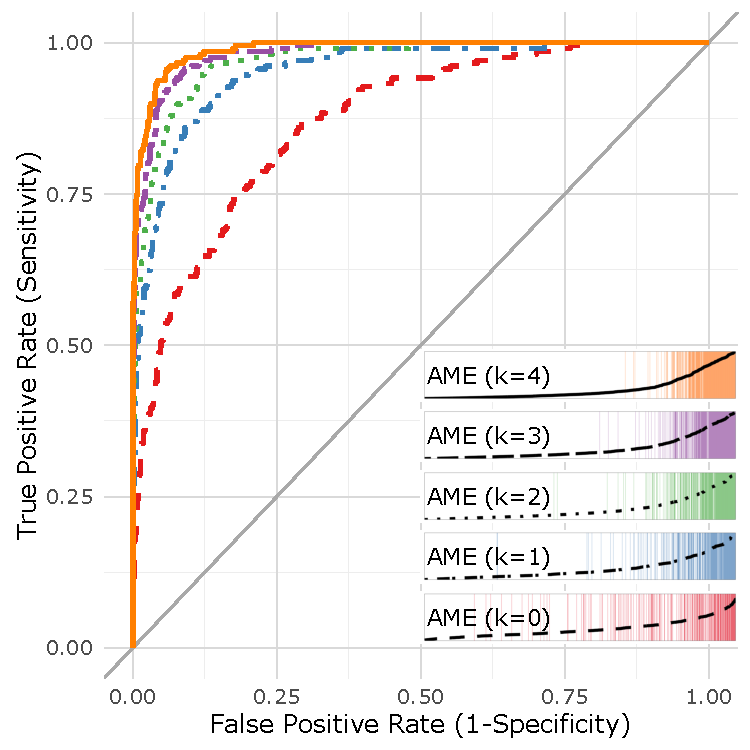
\includegraphics[width=.5\textwidth]{roc_ame} & 
	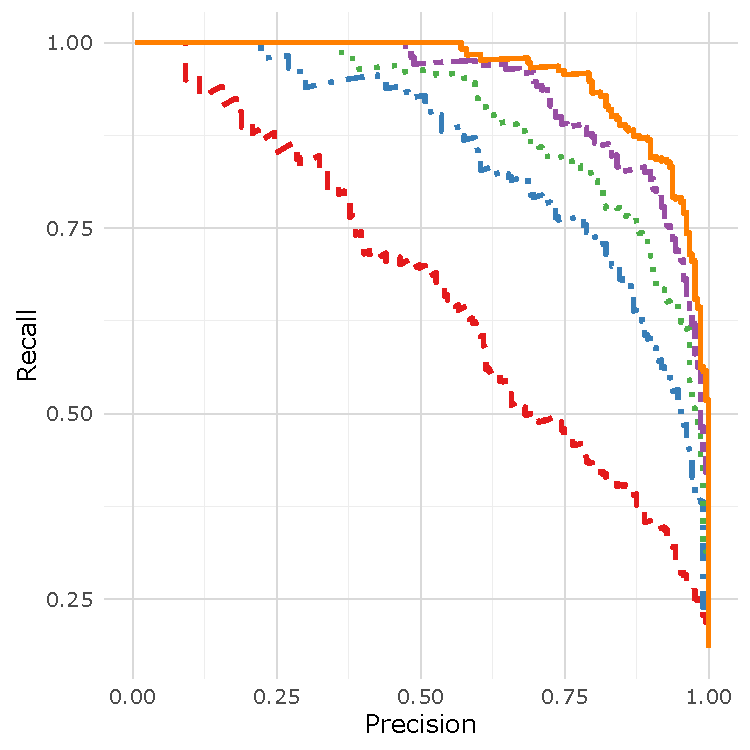
\includegraphics[width=.5\textwidth]{rocPr_ame}
	\end{tabular}
	\caption{ROC and separation plots}
	\label{fig:roc_latentSpace}
\end{figure}

% latex table generated in R 3.3.1 by xtable 1.8-2 package
% Tue Oct 18 00:16:17 2016
\begin{table}[ht]
\centering
\begingroup\normalsize
\begin{tabular}{lcc}
  & AUC & AUC (PR) \\ 
  \hline
\hline
AME (k=4) & 1.00 & 0.98 \\ 
  AME (k=3) & 0.99 & 0.97 \\ 
  AME (k=2) & 0.99 & 0.94 \\ 
  AME (k=1) & 0.97 & 0.90 \\ 
  \end{tabular}
\endgroup
\caption{Area under the curve (AUC) comparison for latent space approaches.} 
\label{tab:aucTable_latSpace}
\end{table}


\begin{figure}[ht]
	\centering
	\begin{tabular}{cc}
	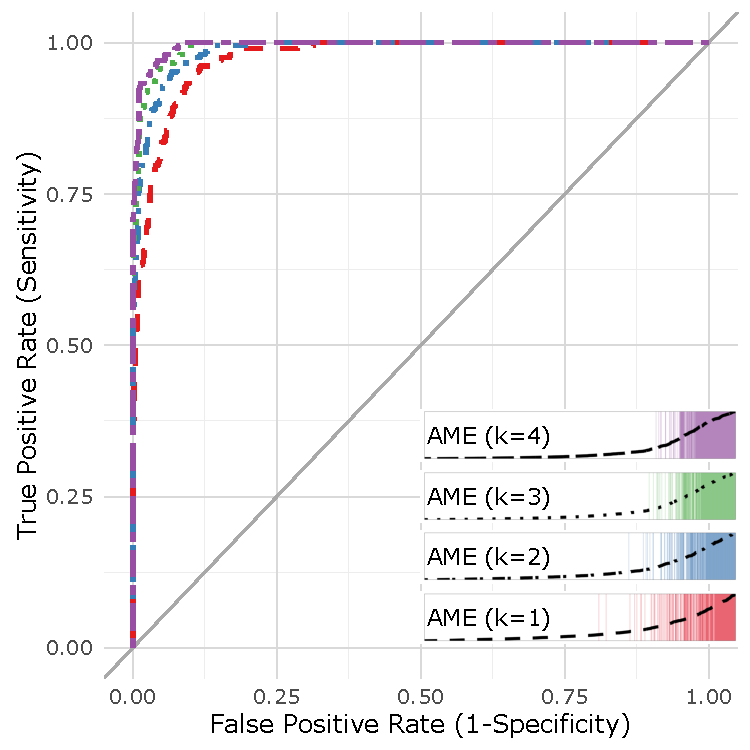
\includegraphics[width=.5\textwidth]{roc_ameSR} & 
	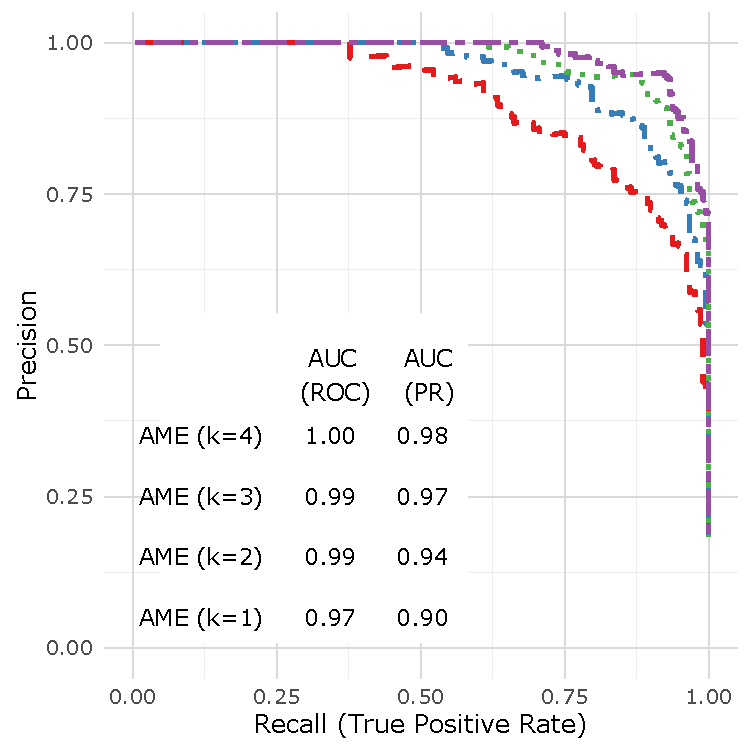
\includegraphics[width=.5\textwidth]{rocPr_ameSR}
	\end{tabular}
	\caption{ROC and separation plots}
	\label{fig:roc_latentSpace}
\end{figure}

\begin{figure}[ht]
	\centering
	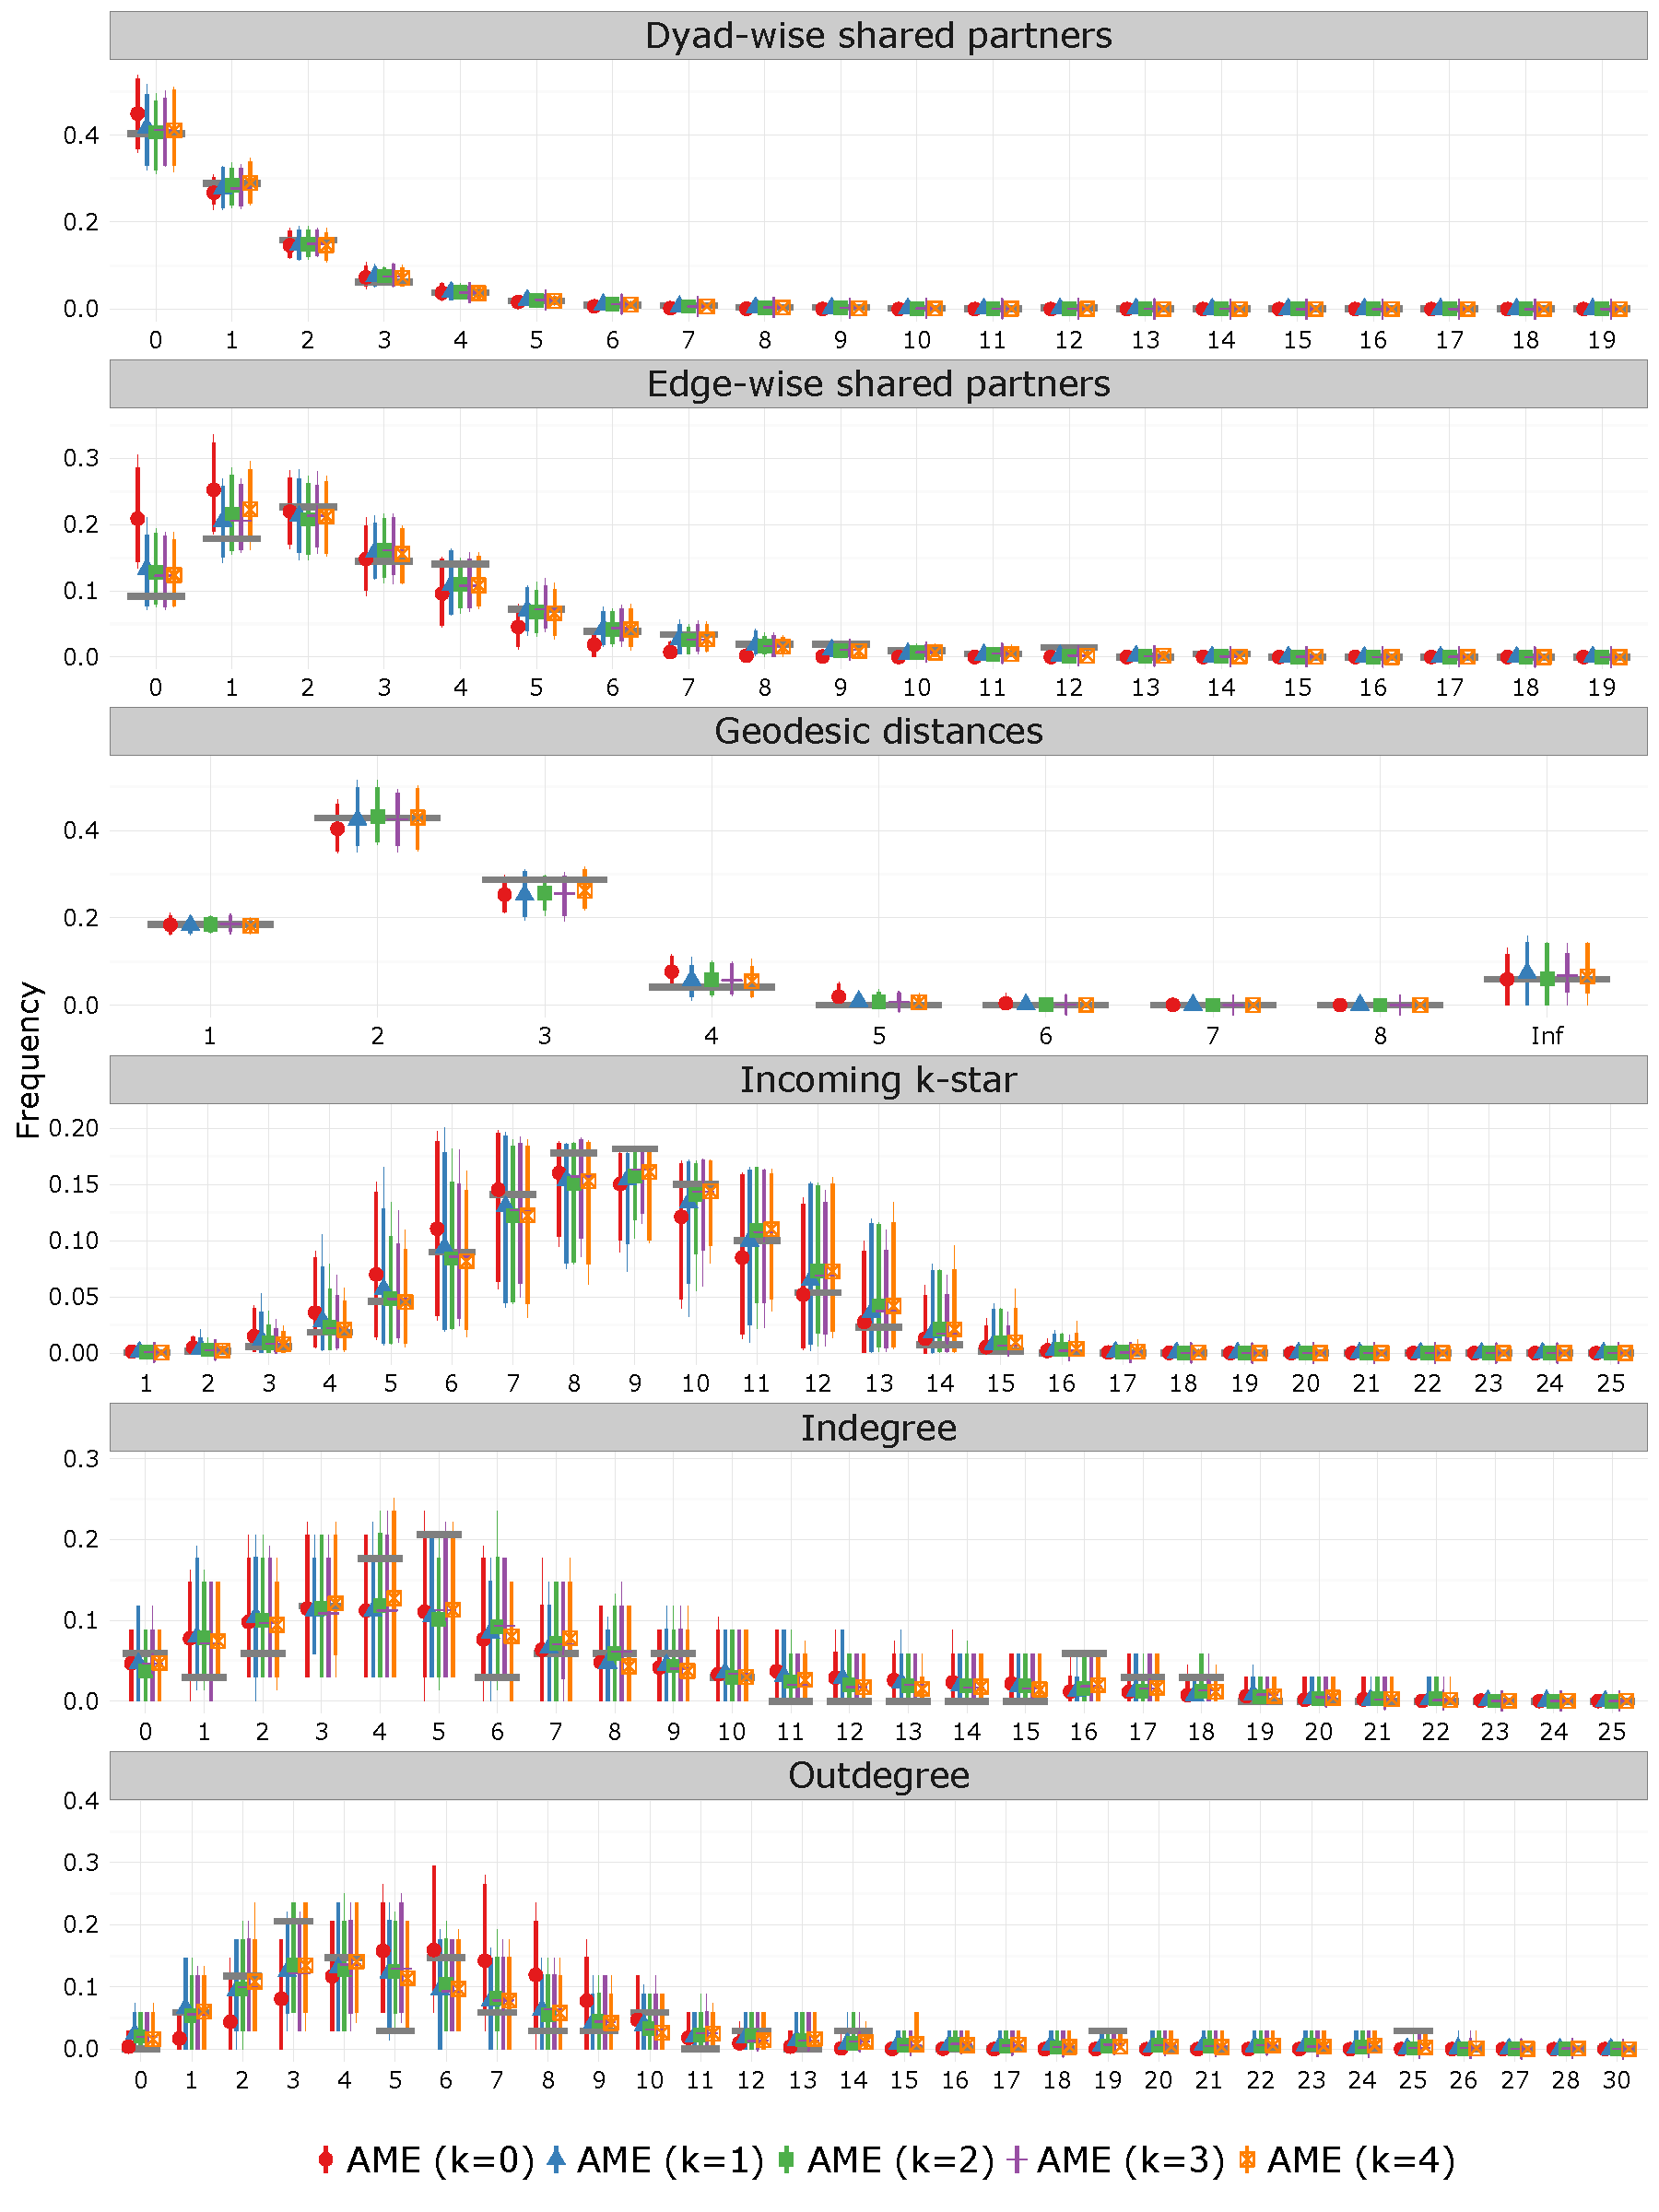
\includegraphics[width=1\textwidth]{ggGofAll_ame}
	\caption{network stats }
	\label{fig:gofAll_ame}
\end{figure}

\begin{figure}[ht]
	\centering
	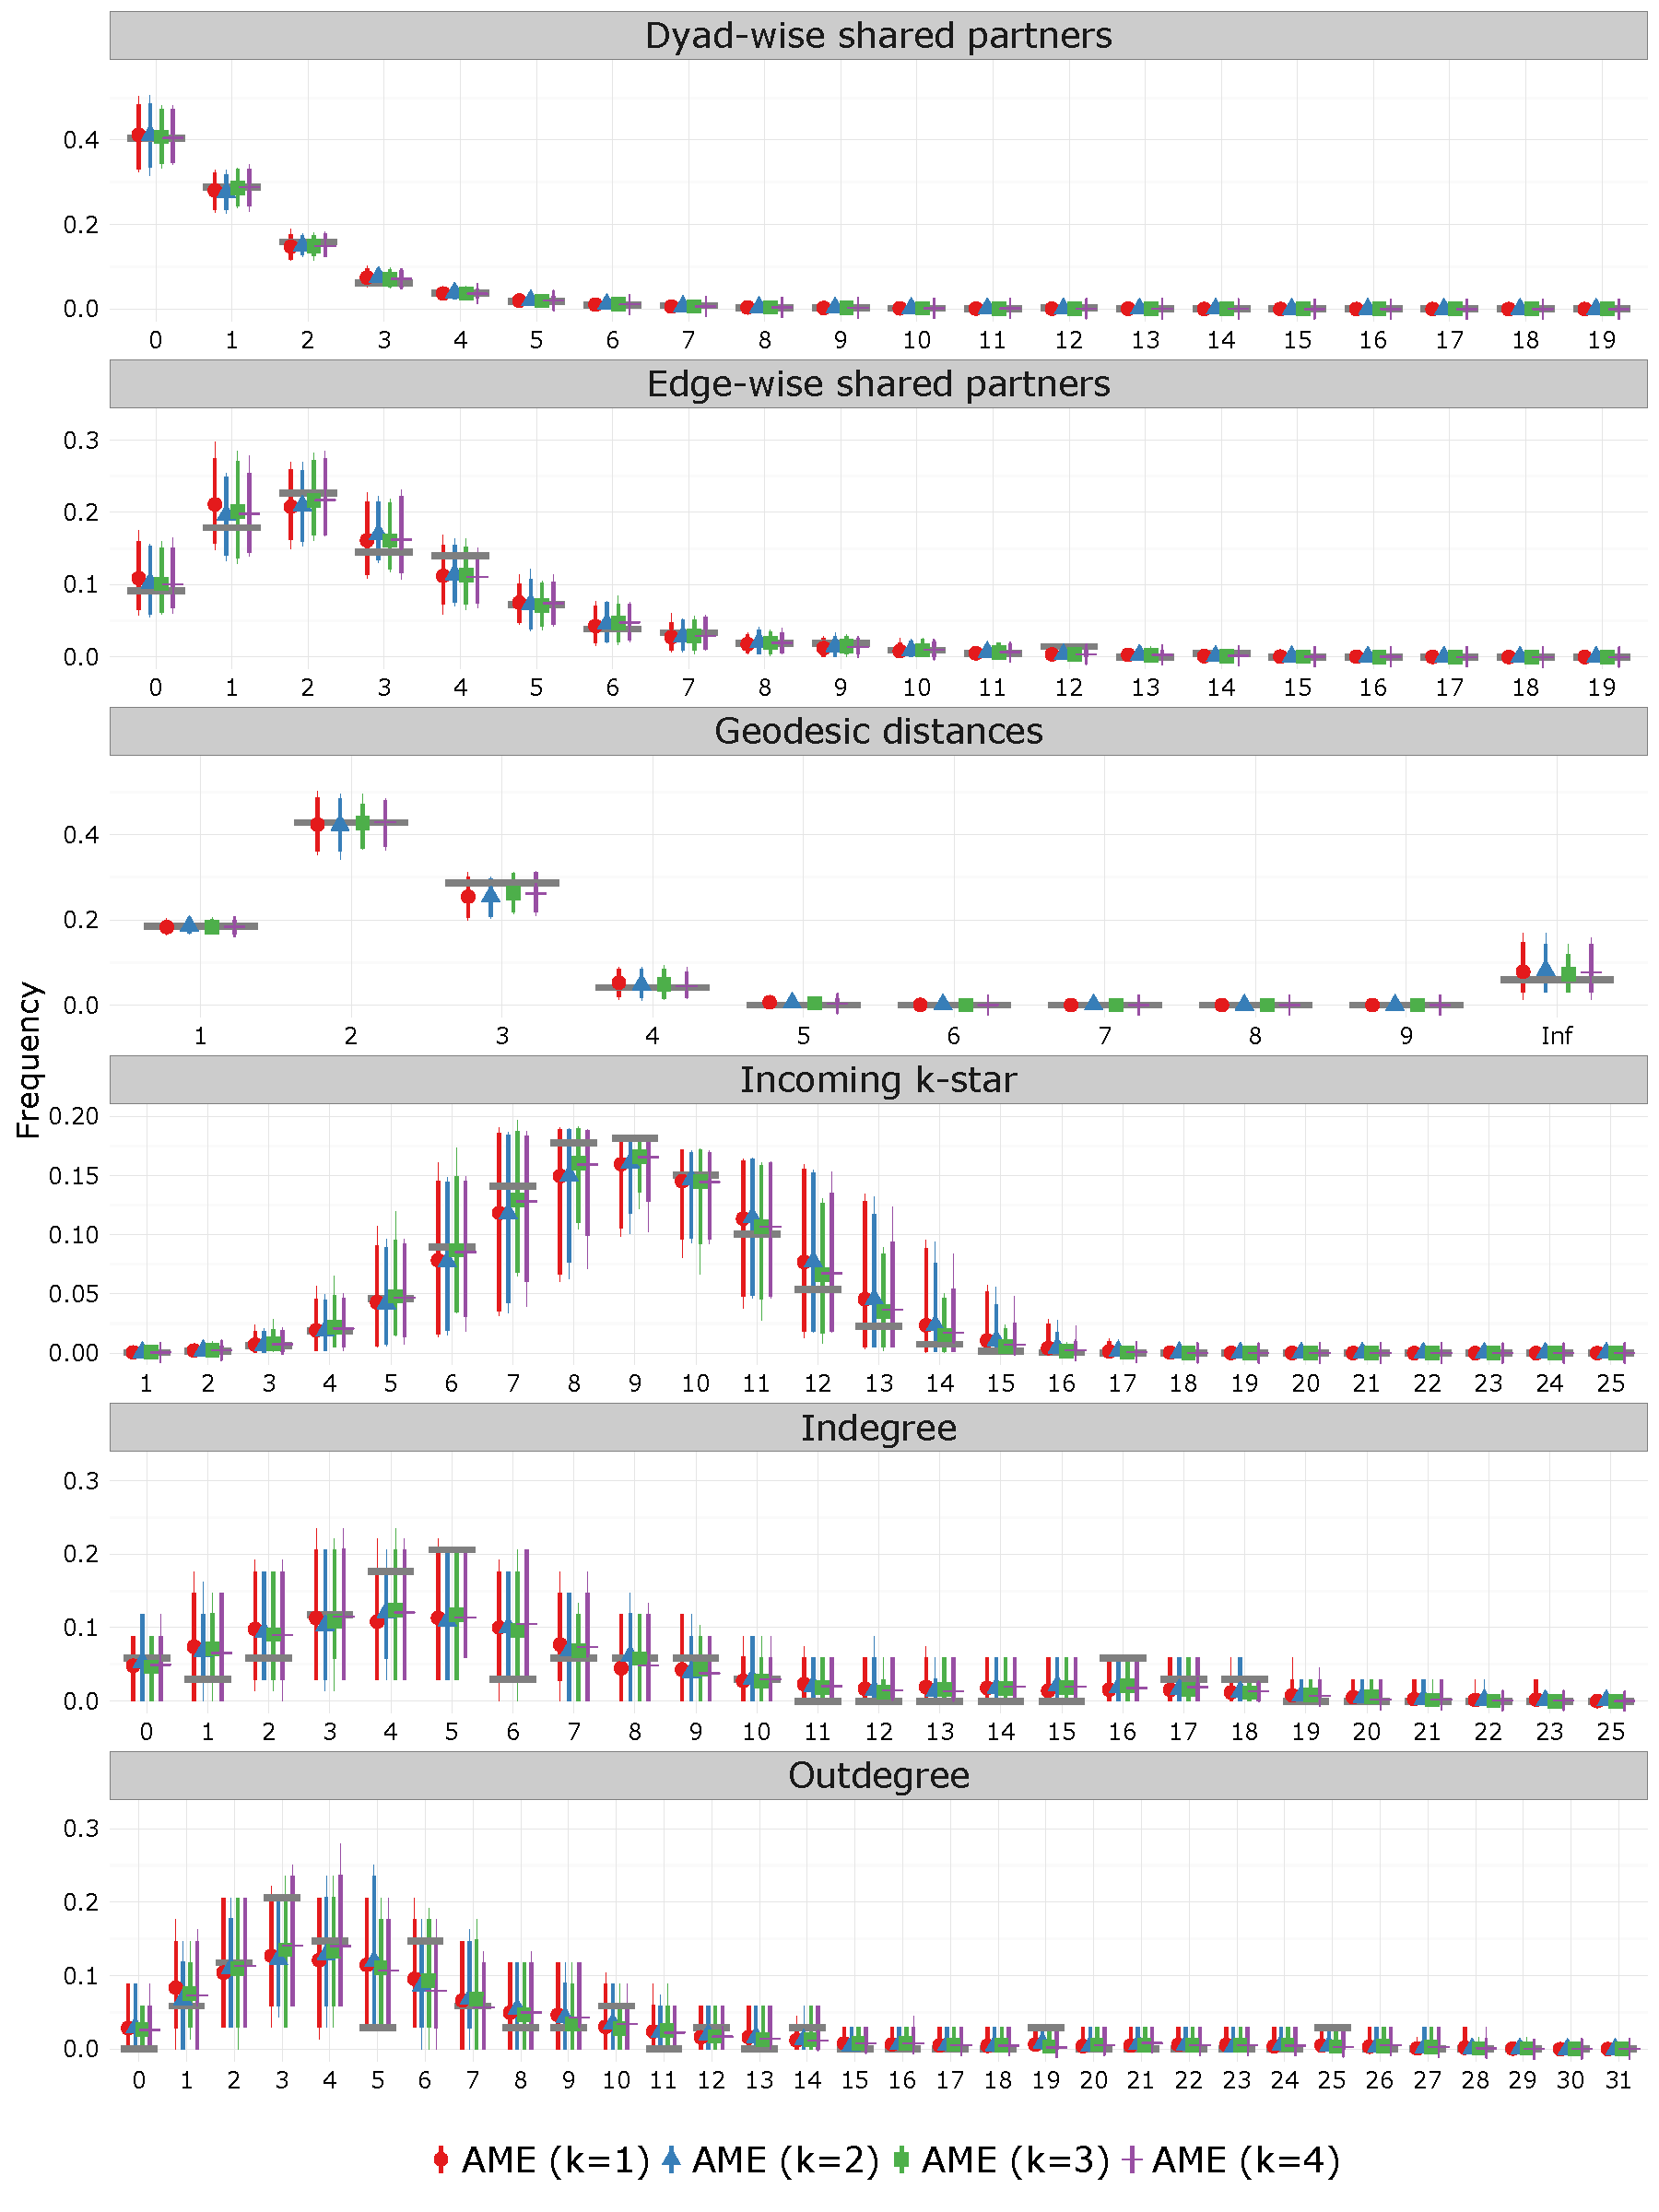
\includegraphics[width=1\textwidth]{ggGofAll_ameSR}
	\caption{network stats }
	\label{fig:gofAll_ameSR}
\end{figure}

\section{Amen \& Latent Net Comparison}
% just in here for now for me to see what's going on with these models

% latex table generated in R 3.3.1 by xtable 1.8-2 package
% Sun Aug 21 03:38:39 2016
\begin{table}[ht]
\centering
\begingroup\tiny
\begin{tabular}{lccccc}
   & LSM & LSM (Bilinear) & LSM (SR) & LSM (Bilinear + SR) & AME \\ 
  \hline
\hline
Intercept/Edges & 0.94$^{\ast}$ & -2.66$^{\ast}$ & 0.60 & -2.50$^{\ast}$ & -3.39$^{\ast}$ \\ 
   & [0.09; 1.82] & [-3.53; -1.87] & [-1.10; 2.37] & [-4.14; -0.88] & [-4.38; -2.50] \\ 
  \textbf{Conflicting policy preferences} &  &  &  &  &  \\ 
  $\;\;\;\;$ Business vs. NGO & -1.37$^{\ast}$ & -2.64$^{\ast}$ & -3.07$^{\ast}$ & -2.87$^{\ast}$ & -1.37$^{\ast}$ \\ 
   & [-2.42; -0.41] & [-4.61; -0.96] & [-4.77; -1.56] & [-4.63; -1.29] & [-2.44; -0.47] \\ 
  $\;\;\;\;$ Opposition/alliance & 0.00 & 0.04 & 0.31 & 0.24 & 1.08$^{\ast}$ \\ 
   & [-0.40; 0.39] & [-0.44; 0.54] & [-0.24; 0.86] & [-0.36; 0.82] & [0.72; 1.47] \\ 
  $\;\;\;\;$ Preference dissimilarity & -1.76$^{\ast}$ & -2.00$^{\ast}$ & -1.88$^{\ast}$ & -2.20$^{\ast}$ & -0.79$^{\ast}$ \\ 
   & [-2.62; -0.90] & [-3.01; -1.03] & [-3.07; -0.68] & [-3.46; -0.96] & [-1.55; -0.08] \\ 
  \textbf{Transaction costs} &  &  &  &  &  \\ 
  $\;\;\;\;$ Joint forum participation & 1.51$^{\ast}$ & 1.24$^{\ast}$ & 1.56$^{\ast}$ & 1.62$^{\ast}$ & 0.92$^{\ast}$ \\ 
   & [0.86; 2.17] & [0.53; 1.93] & [0.69; 2.41] & [0.70; 2.52] & [0.40; 1.47] \\ 
  \textbf{Influence} &  &  &  &  &  \\ 
  $\;\;\;\;$ Influence attribution & 0.08 & -0.08 & 0.30 & 0.28 & 1.09$^{\ast}$ \\ 
   & [-0.40; 0.55] & [-0.62; 0.46] & [-0.37; 0.96] & [-0.42; 0.97] & [0.69; 1.53] \\ 
  $\;\;\;\;$ Alter's influence indegree & 0.01 & -0.05$^{\ast}$ & 0.06 & 0.05 & 0.11$^{\ast}$ \\ 
   & [-0.03; 0.04] & [-0.09; -0.01] & [-0.03; 0.14] & [-0.04; 0.13] & [0.07; 0.15] \\ 
  $\;\;\;\;$ Influence absolute diff. & 0.04 & 0.02 & -0.08$^{\ast}$ & -0.08$^{\ast}$ & -0.07$^{\ast}$ \\ 
   & [-0.01; 0.09] & [-0.03; 0.07] & [-0.14; -0.02] & [-0.14; -0.02] & [-0.11; -0.03] \\ 
  $\;\;\;\;$ Alter = Government actor & -0.46 & -0.80 & -0.11 & -0.20 & 0.55 \\ 
   & [-1.08; 0.14] & [-1.67; 0.04] & [-1.91; 1.76] & [-2.14; 1.74] & [-0.07; 1.15] \\ 
  \textbf{Functional requirements} &  &  &  &  &  \\ 
  $\;\;\;\;$ Ego = Environmental NGO & -0.60 & -1.90$^{\ast}$ & -1.69 & -1.84 & 0.67 \\ 
   & [-1.32; 0.09] & [-3.10; -0.86] & [-3.74; 0.23] & [-4.02; 0.11] & [-0.38; 1.71] \\ 
  $\;\;\;\;$ Same actor type & 1.17$^{\ast}$ & 1.40$^{\ast}$ & 1.82$^{\ast}$ & 1.90$^{\ast}$ & 1.04$^{\ast}$ \\ 
   & [0.63; 1.71] & [0.85; 1.95] & [1.10; 2.54] & [1.19; 2.62] & [0.63; 1.50] \\ 
   \hline
\hline
\end{tabular}
\endgroup
\caption{* p $<$ 0.05. 95\% posterior credible intervals are provided in brackets.} 
\label{tab:regTable_latSpace}
\end{table}


% latex table generated in R 3.3.1 by xtable 1.8-2 package
% Tue Oct 18 00:16:32 2016
\begin{table}[ht]
\centering
\begingroup\normalsize
\begin{tabular}{lcc}
  & AUC & AUC (PR) \\ 
  \hline
\hline
AME & 0.99 & 0.94 \\ 
  LSM (Bilinear + SR) & 0.97 & 0.91 \\ 
  LSM (SR) & 0.97 & 0.90 \\ 
  LSM (Bilinear) & 0.93 & 0.77 \\ 
  LSM & 0.92 & 0.68 \\ 
  \end{tabular}
\endgroup
\caption{Area under the curve (AUC) comparison for latent space approaches.} 
\label{tab:aucTable_latSpace}
\end{table}


\begin{figure}[ht]
	\centering
	\begin{tabular}{cc}
	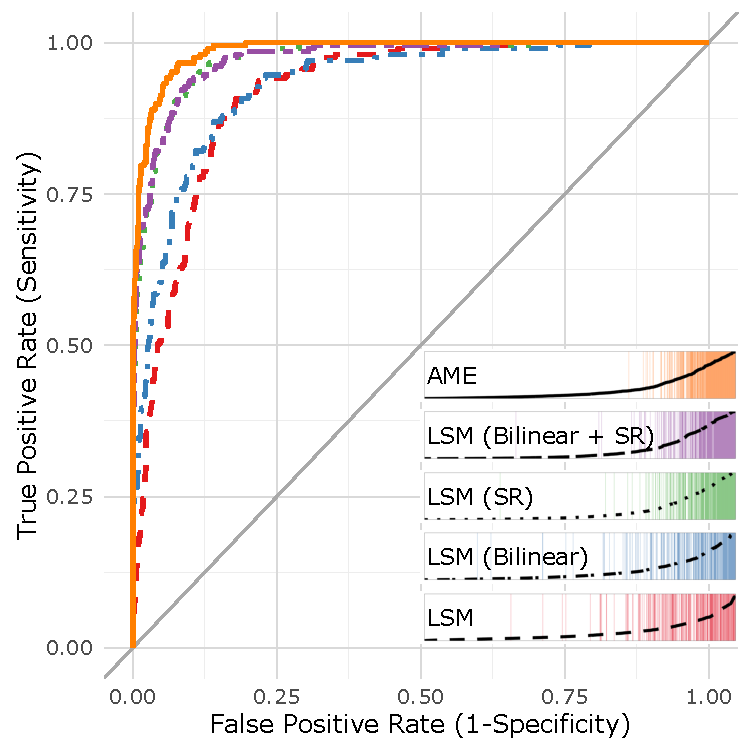
\includegraphics[width=.5\textwidth]{roc_latSpace} & 
	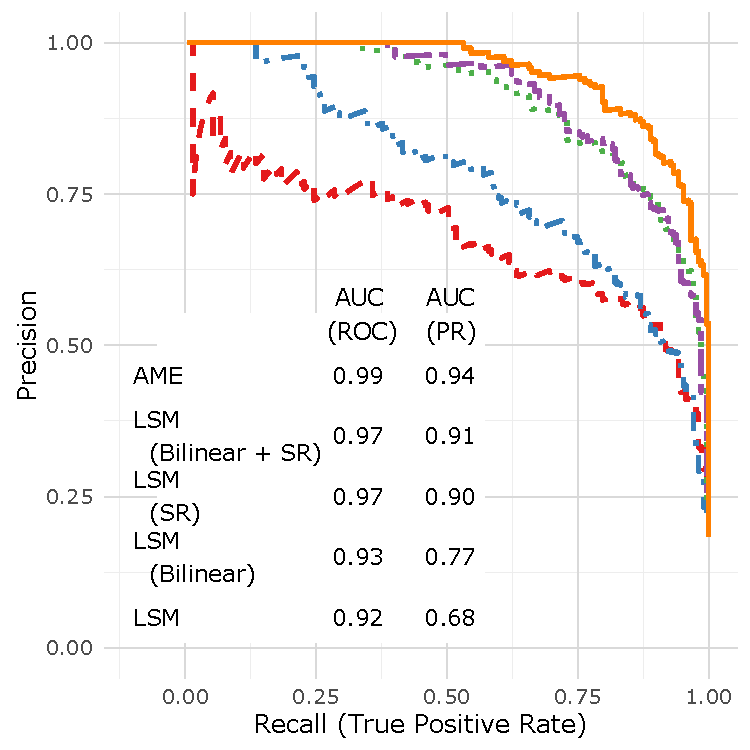
\includegraphics[width=.5\textwidth]{rocPr_latSpace}
	\end{tabular}
	\caption{ROC and separation plots}
	\label{fig:roc_latentSpace}
\end{figure}

\begin{figure}[ht]
	\centering
	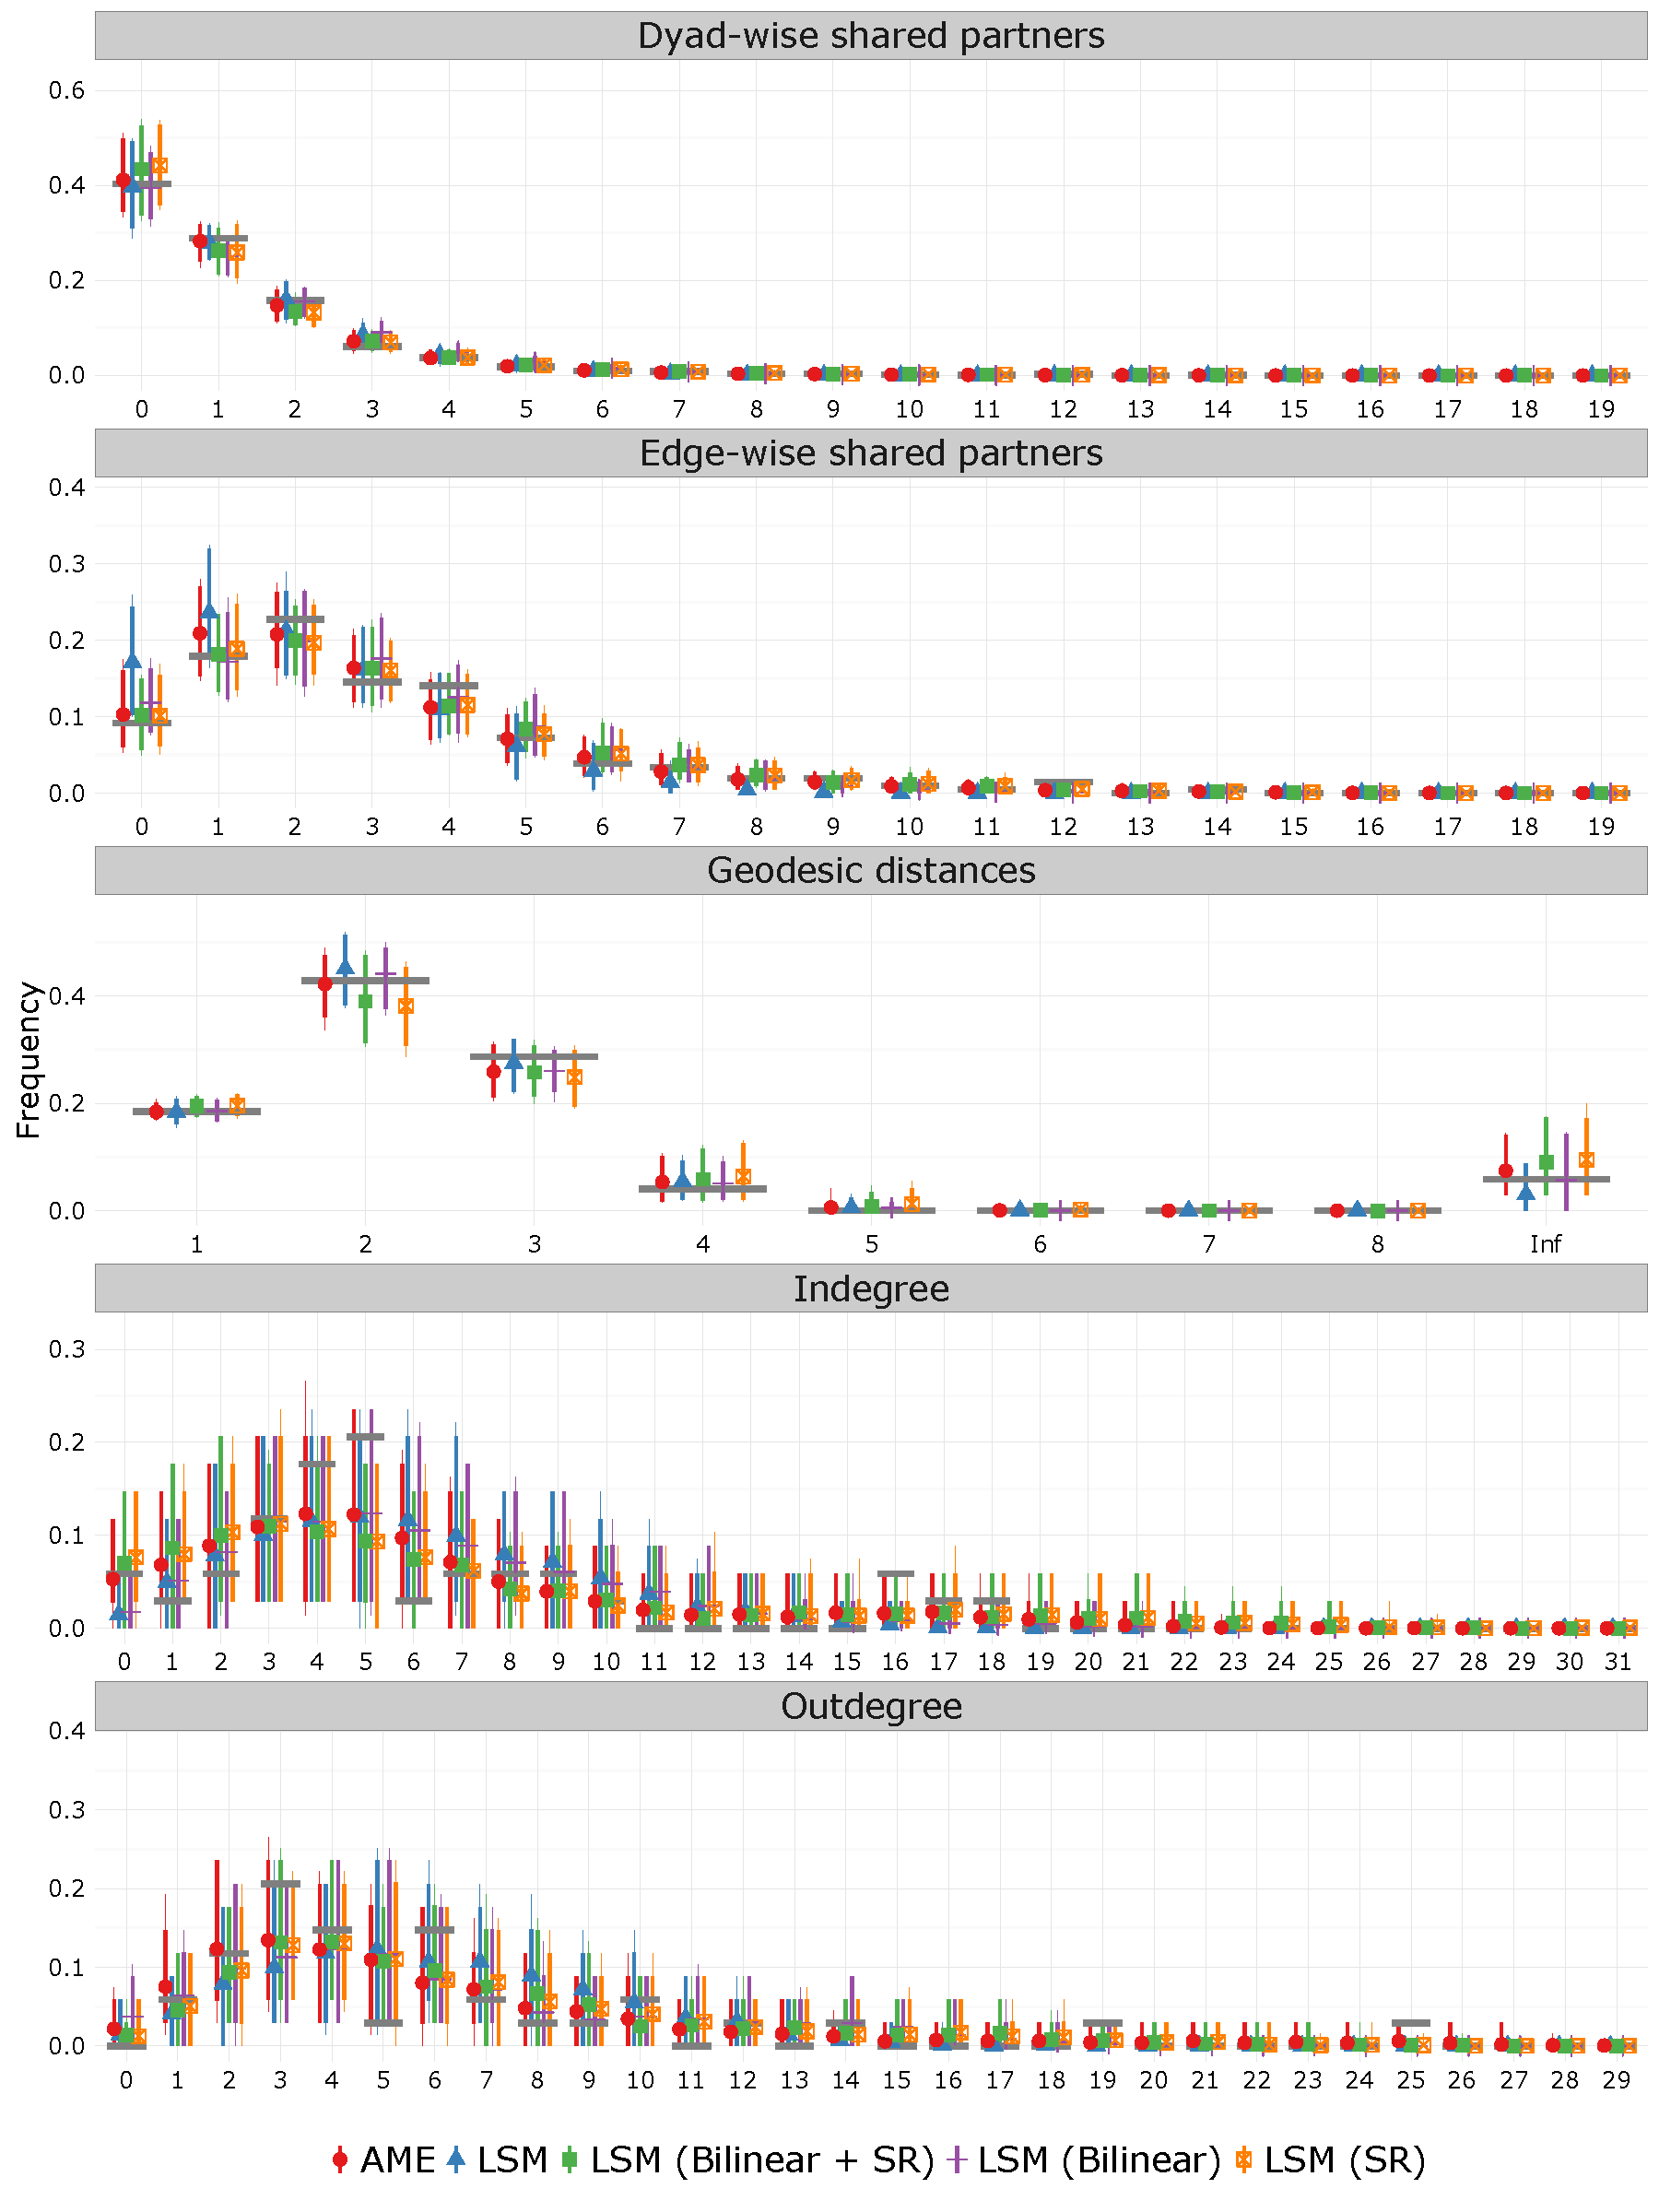
\includegraphics[width=1\textwidth]{ggGofAll_latSpace}
	\caption{network stats }
	\label{fig:gofAll_latSpace}
\end{figure}

\newpage

% \lstinputlisting{../combinedData.R}
\bibliography{/Users/janus829/Documents/references.bib}

\end{document} 